\chapter{Benchmarks}

I benchmark sono stati eseguiti su due configurazioni di magazzino (Preset~A e Preset~B)
con lo stesso numero di run per garantire significativit\`a statistica.
Per ogni preset vengono riportati quattro grafici e una tabella riepilogativa.

\section*{Configurazioni di test}

Ogni esecuzione \`e identificata da un'etichetta composta che riflette tre assi di variazione
ortogonali, applicati in modo identico a entrambi i preset.

\paragraph{Composizione degli agenti.}
La notazione \texttt{$x$S-$y$C-$z$R} indica il numero di Scout (\textbf{S}), Coordinator
(\textbf{C}) e Retriever (\textbf{R}) presenti nella simulazione.
Sono state testate due composizioni:
\begin{itemize}
  \item \textbf{1S-1C-3R} --- configurazione completa con gerarchia di ruoli: uno Scout esplora
        la mappa e riporta le posizioni degli oggetti, un Coordinator raccoglie le segnalazioni
        e assegna i compiti, tre Retriever prelevano e consegnano gli oggetti.
  \item \textbf{0S-0C-5R} --- configurazione \emph{baseline} senza Scout n\'e Coordinator:
        cinque Retriever operano in modo autonomo, scoprendo gli oggetti solo tramite visione
        diretta.
\end{itemize}

\paragraph{Modalit\`a mappa.}
\begin{itemize}
  \item \texttt{unknown} --- gli agenti non conoscono \textit{a priori} la planimetria del
        magazzino; l'ambiente viene scoperto progressivamente (fog-of-war).
  \item \texttt{map\_known} --- la mappa \`e nota fin dall'inizio; gli agenti possono
        pianificare percorsi ottimali senza dover esplorare.
\end{itemize}

\paragraph{Comportamento \texttt{seek\_coordinator}.}
Nelle configurazioni con Scout, il flag \texttt{seek\_coordinator} (attivo per default) fa s\'i
che lo Scout, dopo un periodo di isolamento, diriga autonomamente verso l'ultima posizione nota
del Coordinator per consegnare le scoperte.
Le varianti con suffisso \textbf{no-seek} disabilitano questo comportamento: lo Scout consegna
le informazioni \emph{solo} quando il Coordinator entra nel suo raggio di comunicazione.

\paragraph{Raggio aumentato ($v_r\!=\!3,\,c_r\!=\!3$).}
Le varianti con suffisso \textbf{v3c3} aumentano a~3 il raggio di visione e di comunicazione
di \emph{tutti} gli agenti (il default varia per ruolo: Scout $v_r\!=\!3$/$c_r\!=\!2$,
Coordinator $v_r\!=\!2$/$c_r\!=\!3$, Retriever $v_r\!=\!2$/$c_r\!=\!2$).
Questo scenario ipotetico serve a valutare l'impatto di una maggiore connettivit\`a sulla performance complessiva.

%% ── Preset A ──────────────────────────────────────────────
\section{Preset A}

\begin{figure}[H]
  \centering
  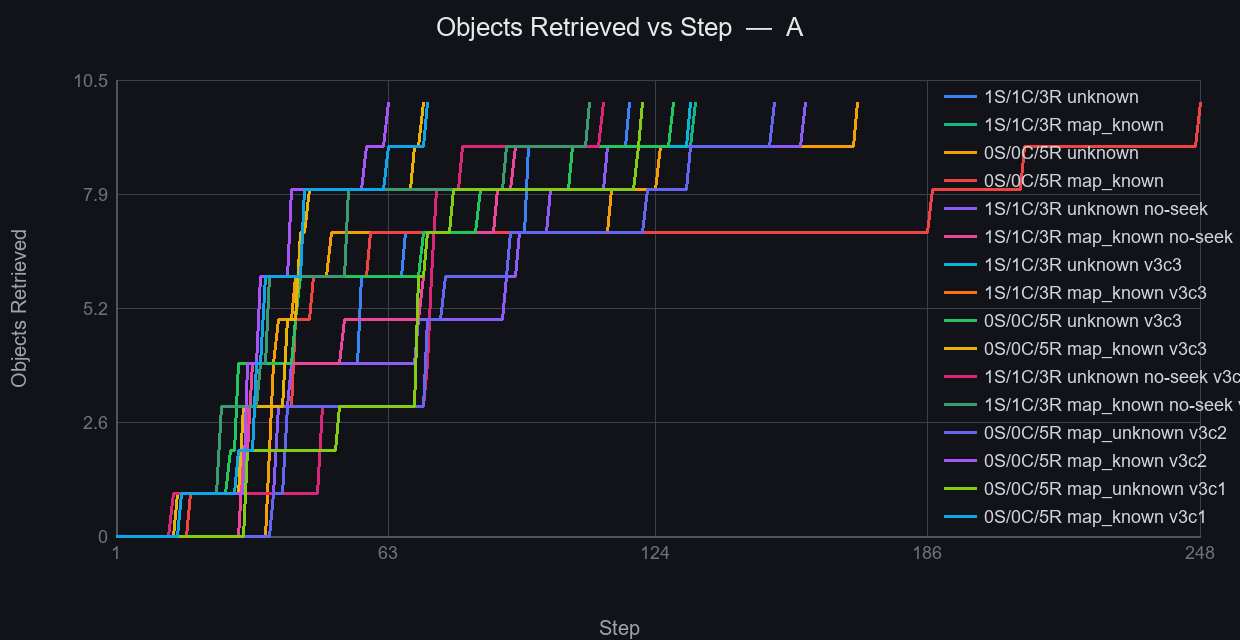
\includegraphics[width=\textwidth]{../benchmarks/A/retrieval.png}
  \caption{Andamento del recupero oggetti --- Preset~A}
  \label{fig:bench-a-retrieval}
\end{figure}

\begin{figure}[H]
  \centering
  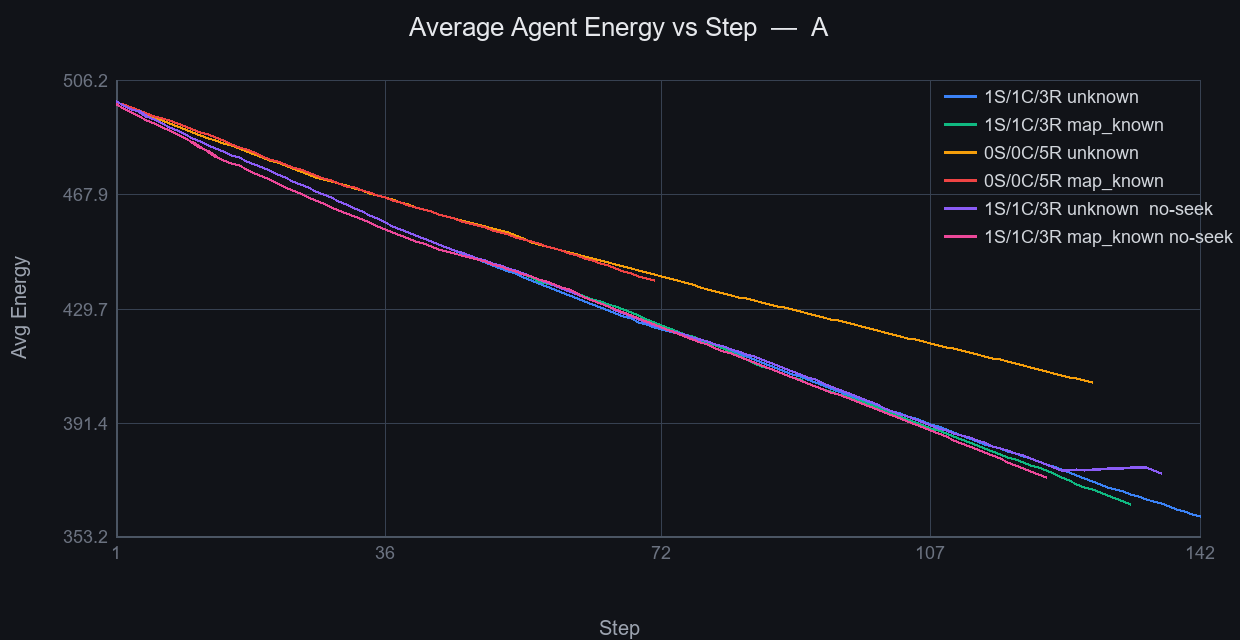
\includegraphics[width=\textwidth]{../benchmarks/A/energy.png}
  \caption{Consumo energetico --- Preset~A}
  \label{fig:bench-a-energy}
\end{figure}

\begin{figure}[H]
  \centering
  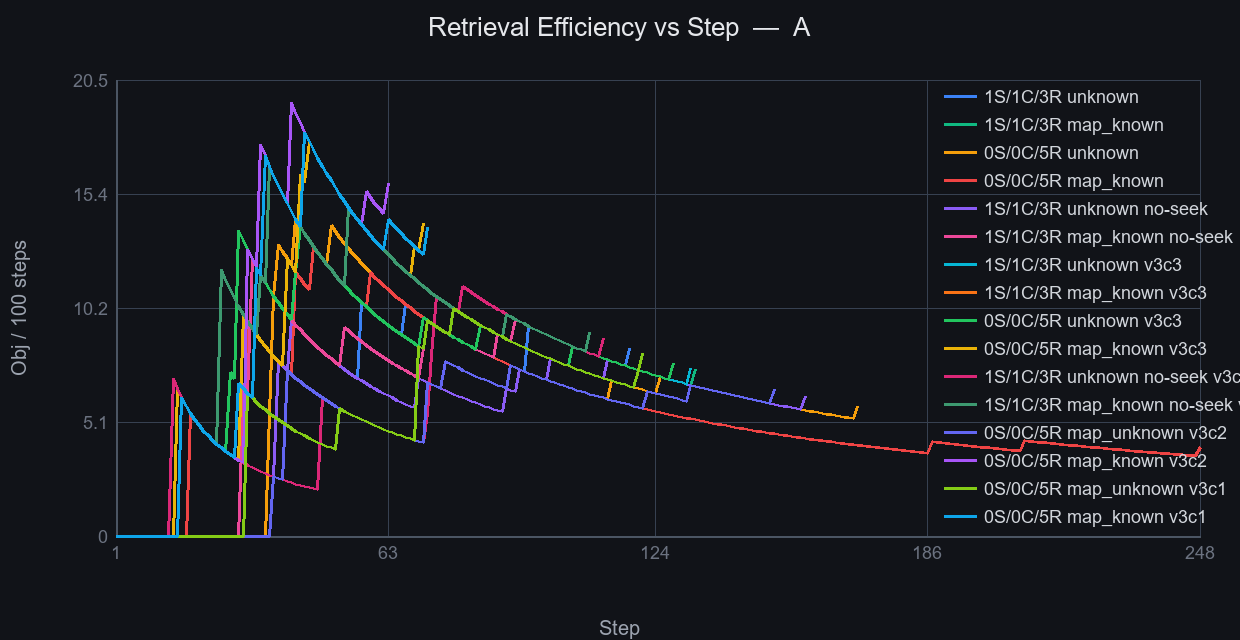
\includegraphics[width=\textwidth]{../benchmarks/A/efficiency.png}
  \caption{Efficienza energetica --- Preset~A}
  \label{fig:bench-a-efficiency}
\end{figure}

\begin{figure}[H]
  \centering
  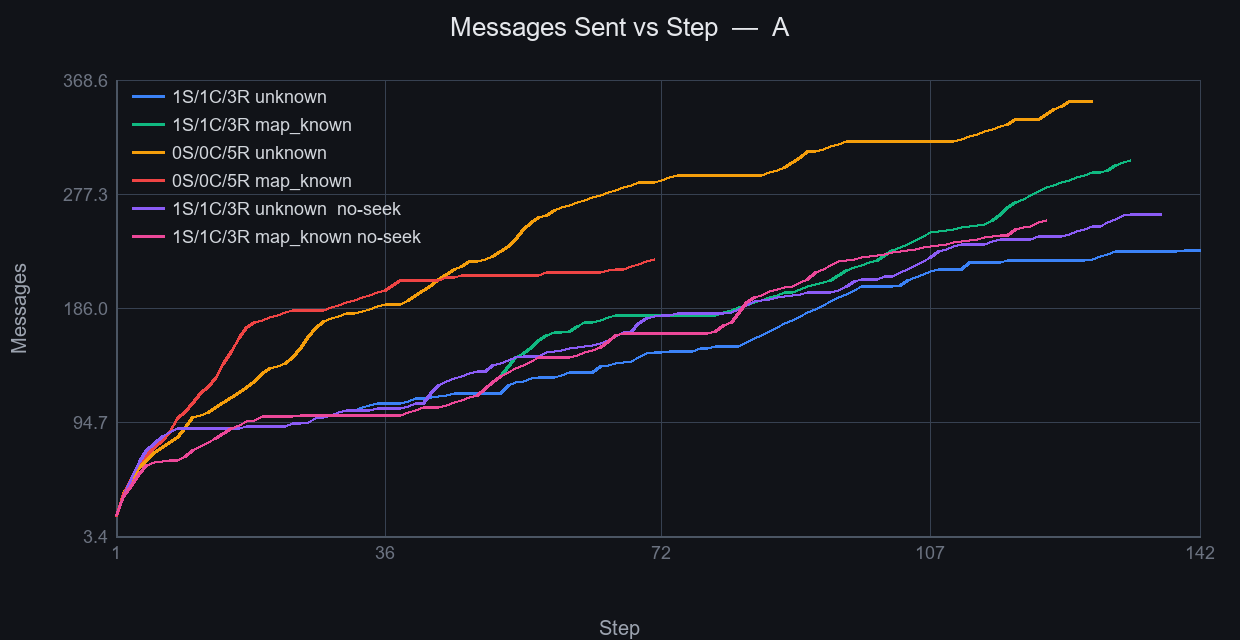
\includegraphics[width=\textwidth]{../benchmarks/A/messages.png}
  \caption{Messaggi scambiati --- Preset~A}
  \label{fig:bench-a-messages}
\end{figure}

\begin{figure}[H]
  \centering
  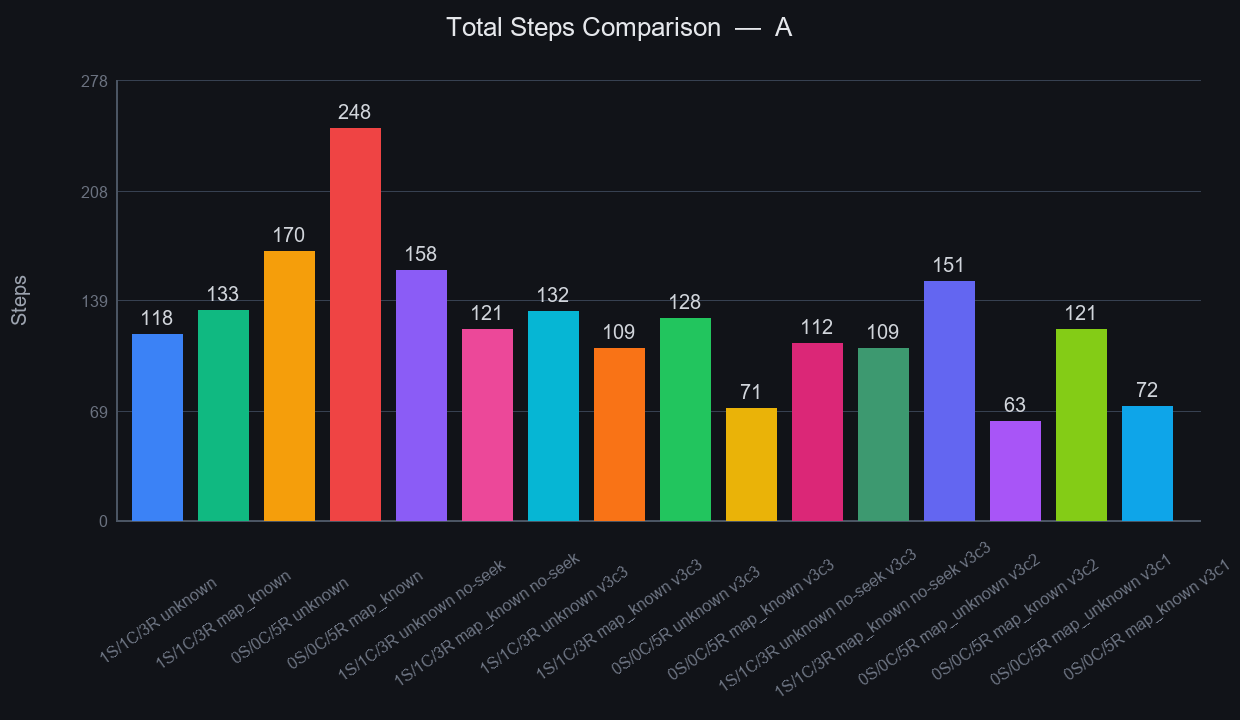
\includegraphics[width=\textwidth]{../benchmarks/A/steps_comparison.png}
  \caption{Confronto step totali --- Preset~A}
  \label{fig:bench-a-steps}
\end{figure}

\begin{figure}[H]
  \centering
  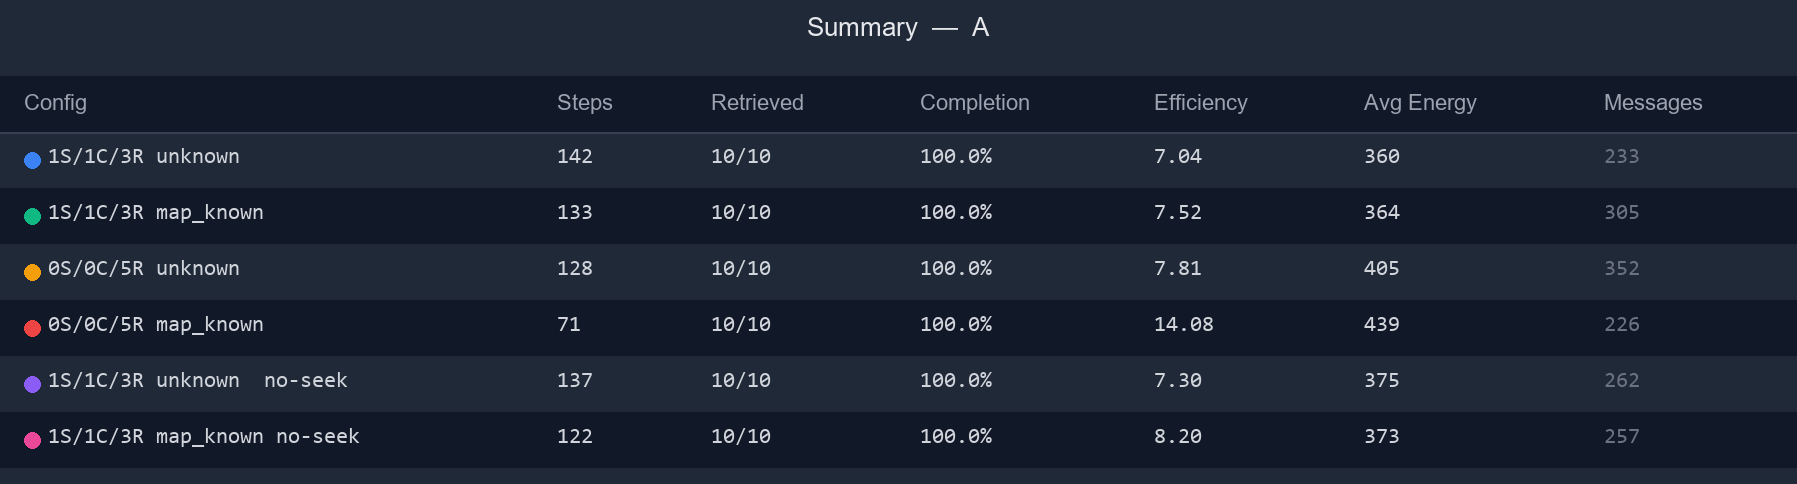
\includegraphics[width=0.92\textwidth]{../benchmarks/A/summary_table.png}
  \caption{Tabella riepilogativa --- Preset~A}
  \label{fig:bench-a-table}
\end{figure}

\subsection{Snapshot Finali --- Preset~A}

\begin{figure}[H]
  \centering
  \subcaptionbox{0S-0C-5R --- \texttt{map\_known}\label{fig:snap-a-05r-mk}}[0.48\textwidth]{%
    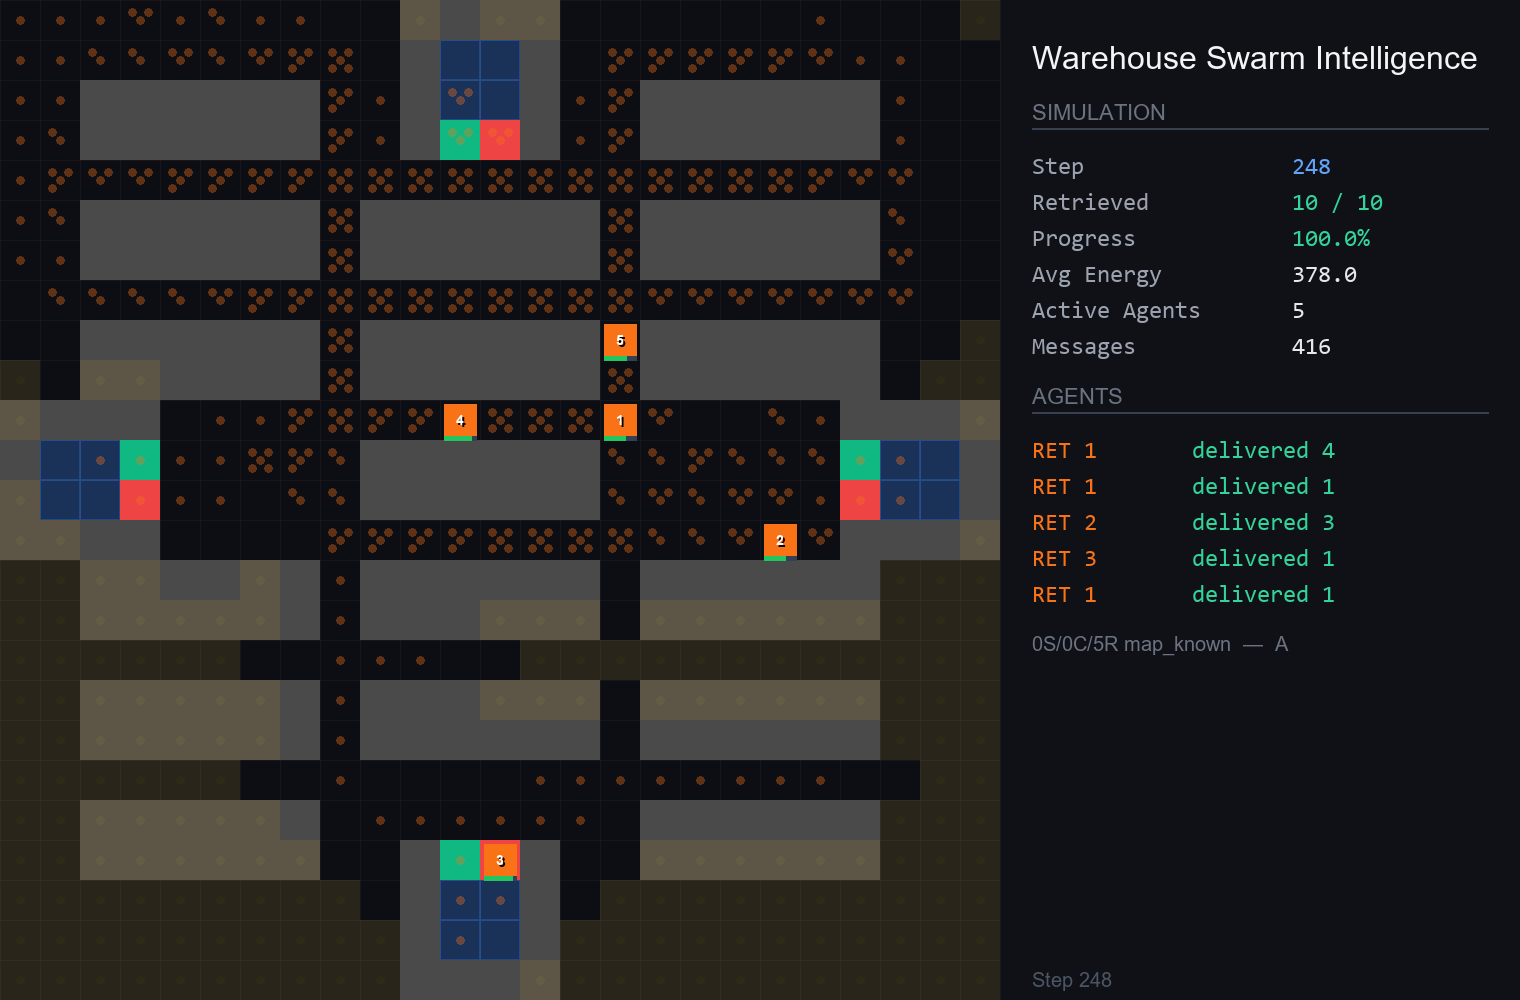
\includegraphics[width=0.48\textwidth]{../benchmarks/A/snapshot_0S-0C-5R_map_known.png}}%
  \hfill
  \subcaptionbox{0S-0C-5R --- \texttt{unknown}\label{fig:snap-a-05r-unk}}[0.48\textwidth]{%
    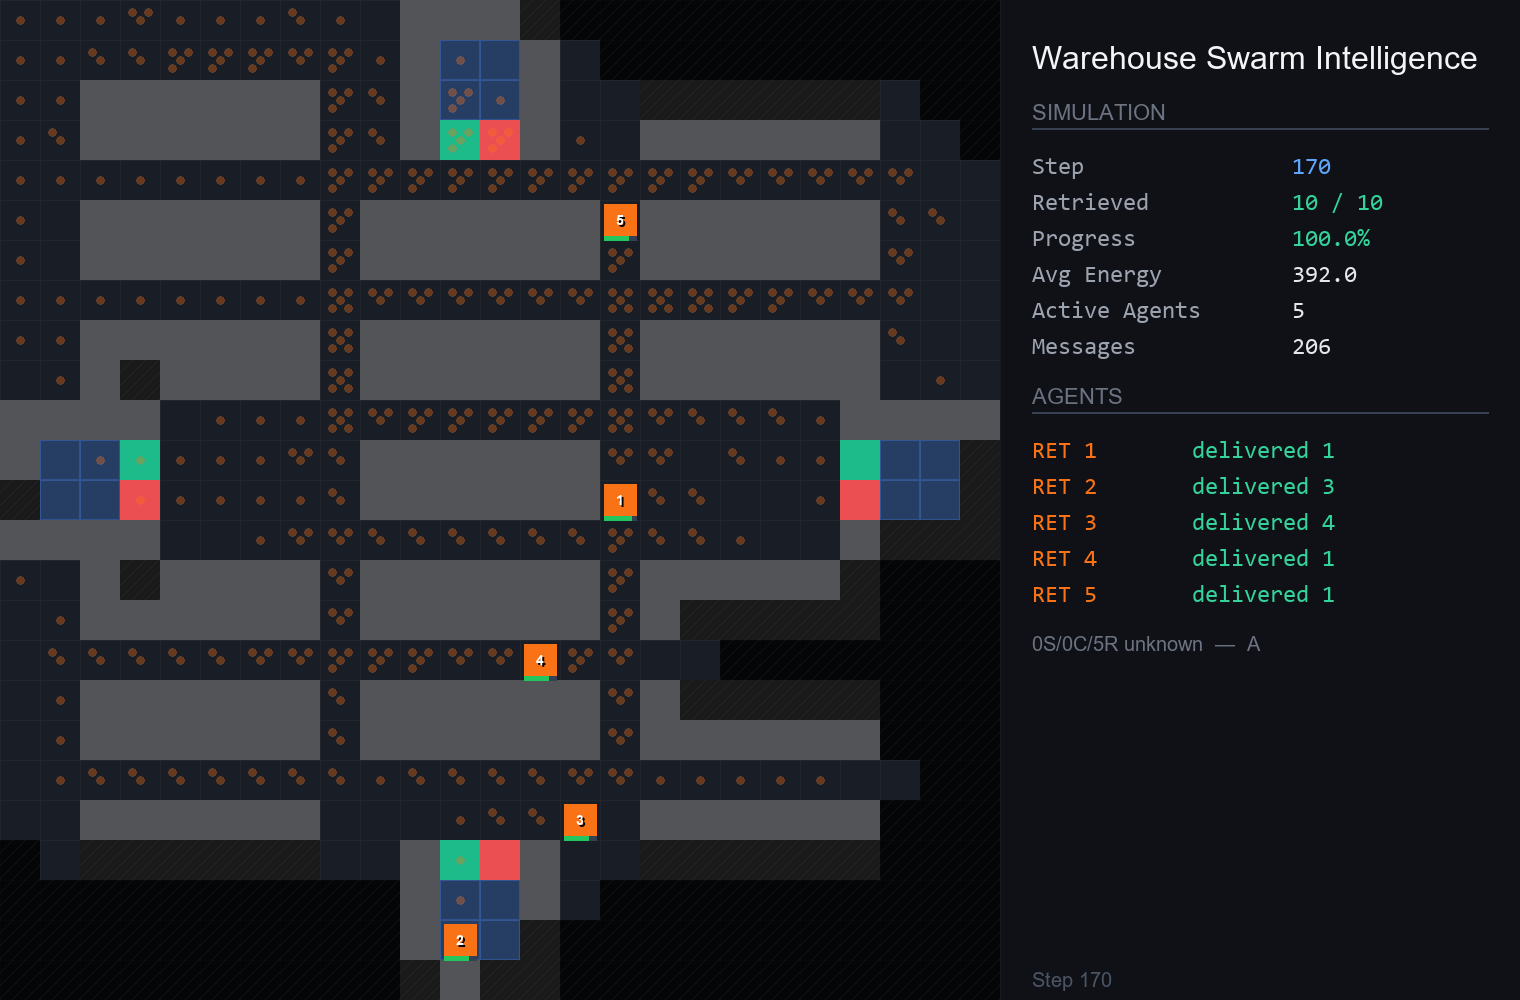
\includegraphics[width=0.48\textwidth]{../benchmarks/A/snapshot_0S-0C-5R_unknown.png}}%
  \\[1ex]
  \subcaptionbox{0S-0C-5R --- \texttt{map\_known}, $v_r\!=\!3,c_r\!=\!3$\label{fig:snap-a-05r-mk-v3c3}}[0.48\textwidth]{%
    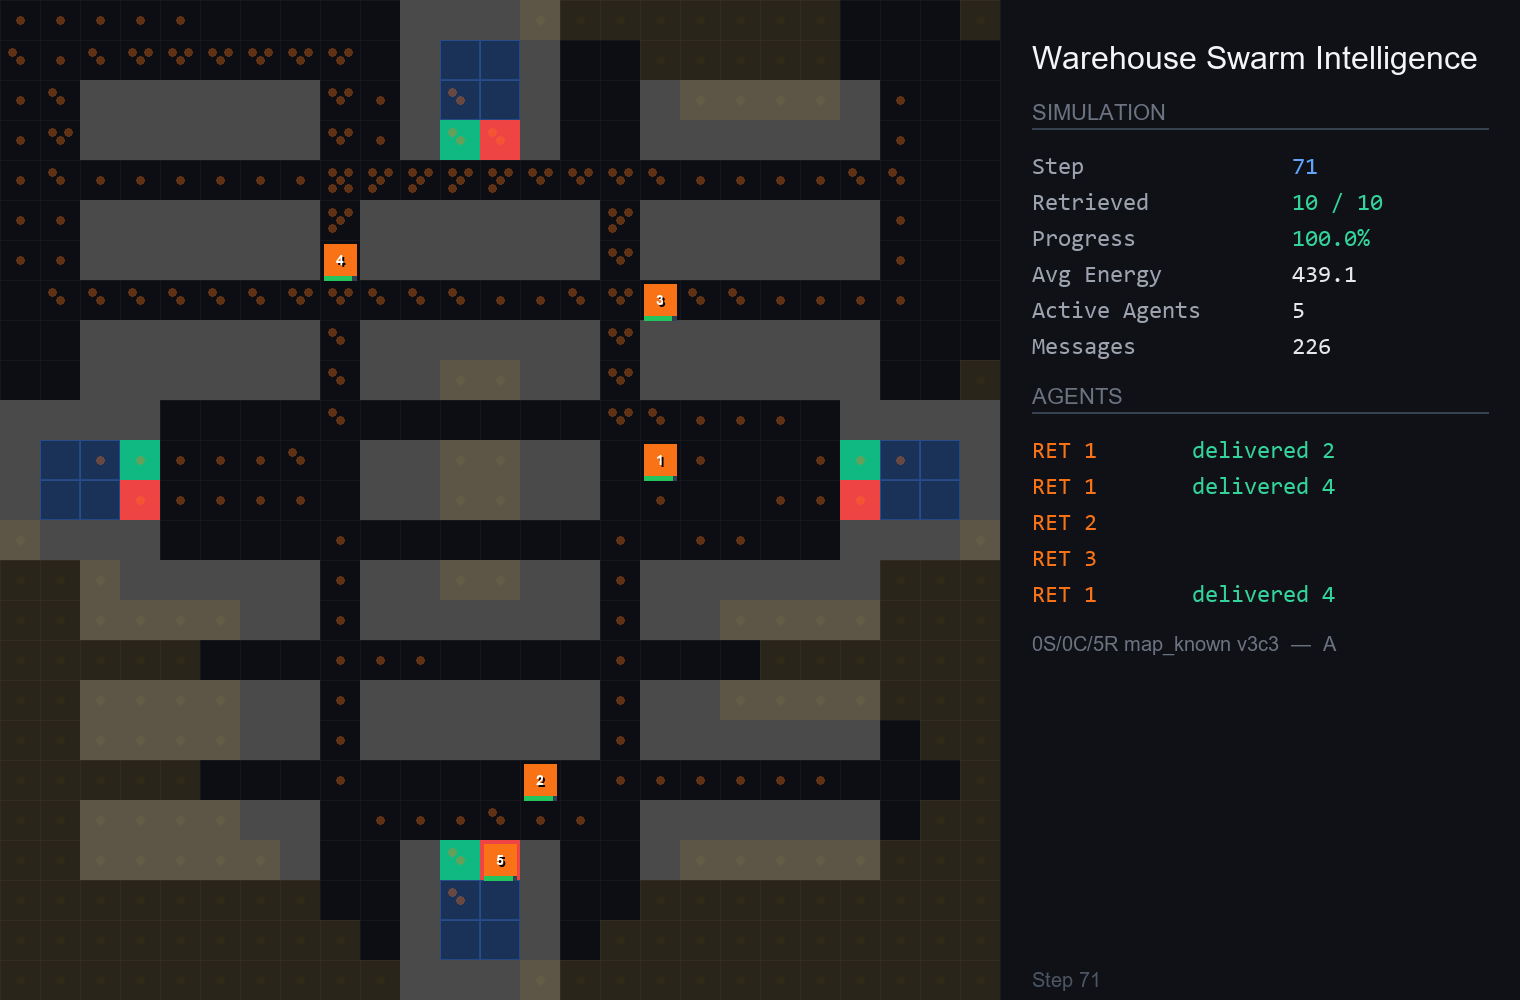
\includegraphics[width=0.48\textwidth]{../benchmarks/A/snapshot_0S-0C-5R_map_known_v3c3.png}}%
  \hfill
  \subcaptionbox{0S-0C-5R --- \texttt{unknown}, $v_r\!=\!3,c_r\!=\!3$\label{fig:snap-a-05r-unk-v3c3}}[0.48\textwidth]{%
    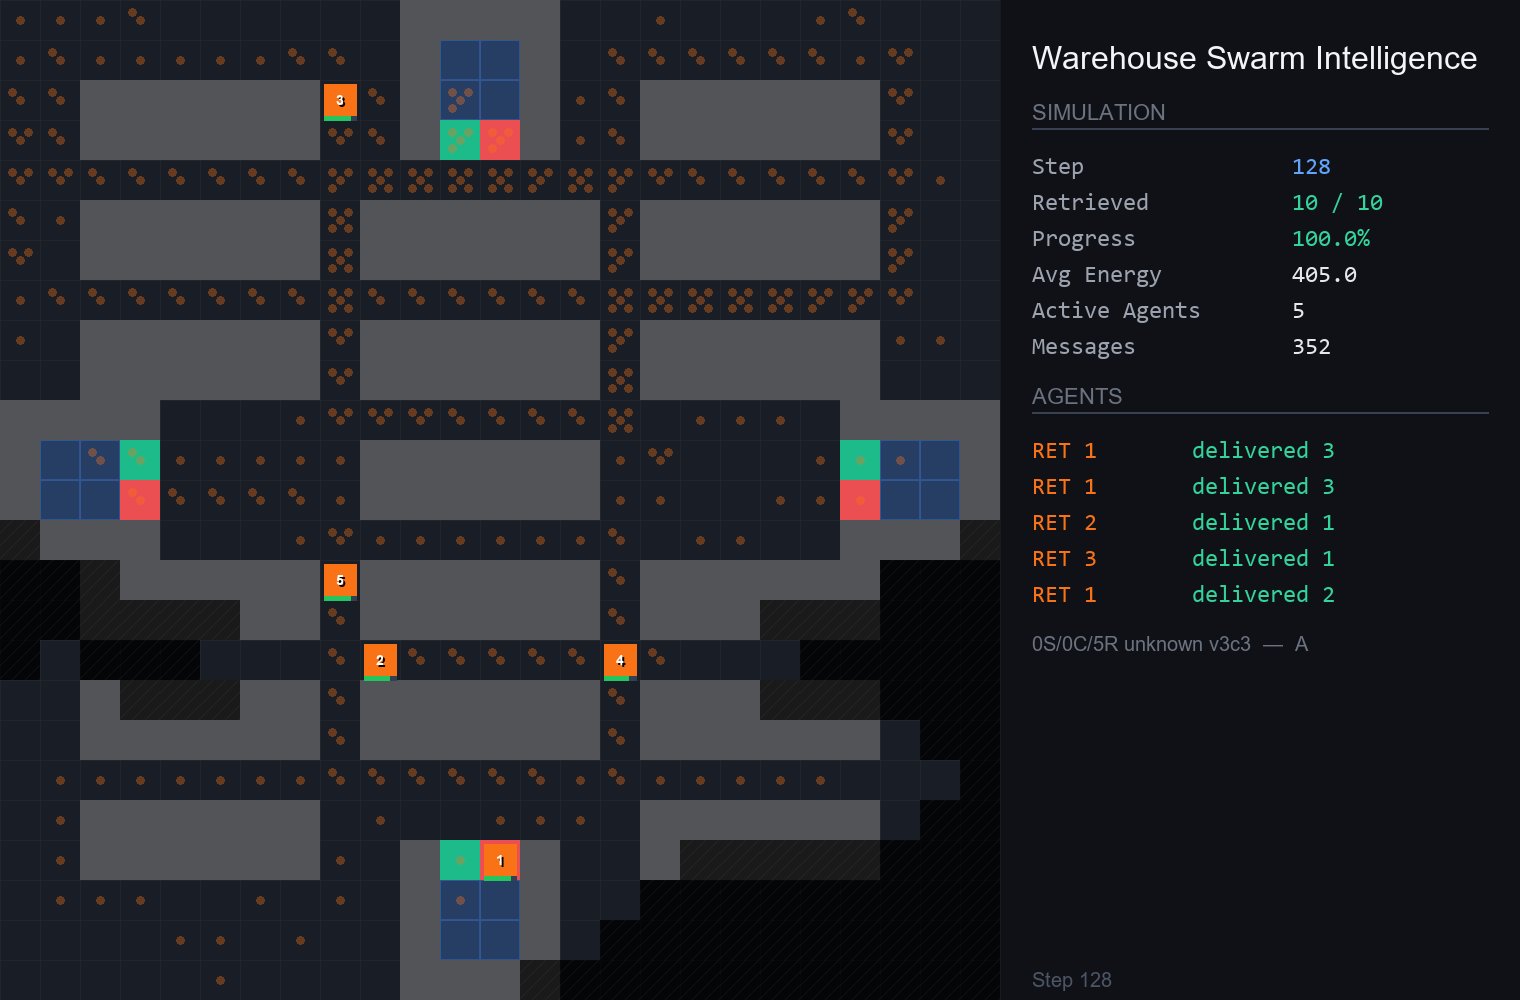
\includegraphics[width=0.48\textwidth]{../benchmarks/A/snapshot_0S-0C-5R_unknown_v3c3.png}}%
  \caption{Snapshot finali --- 0S-0C-5R, Preset~A}
  \label{fig:snap-a-05r}
\end{figure}

\begin{figure}[H]
  \centering
  \subcaptionbox{1S-1C-3R --- \texttt{map\_known}\label{fig:snap-a-13r-mk}}[0.48\textwidth]{%
    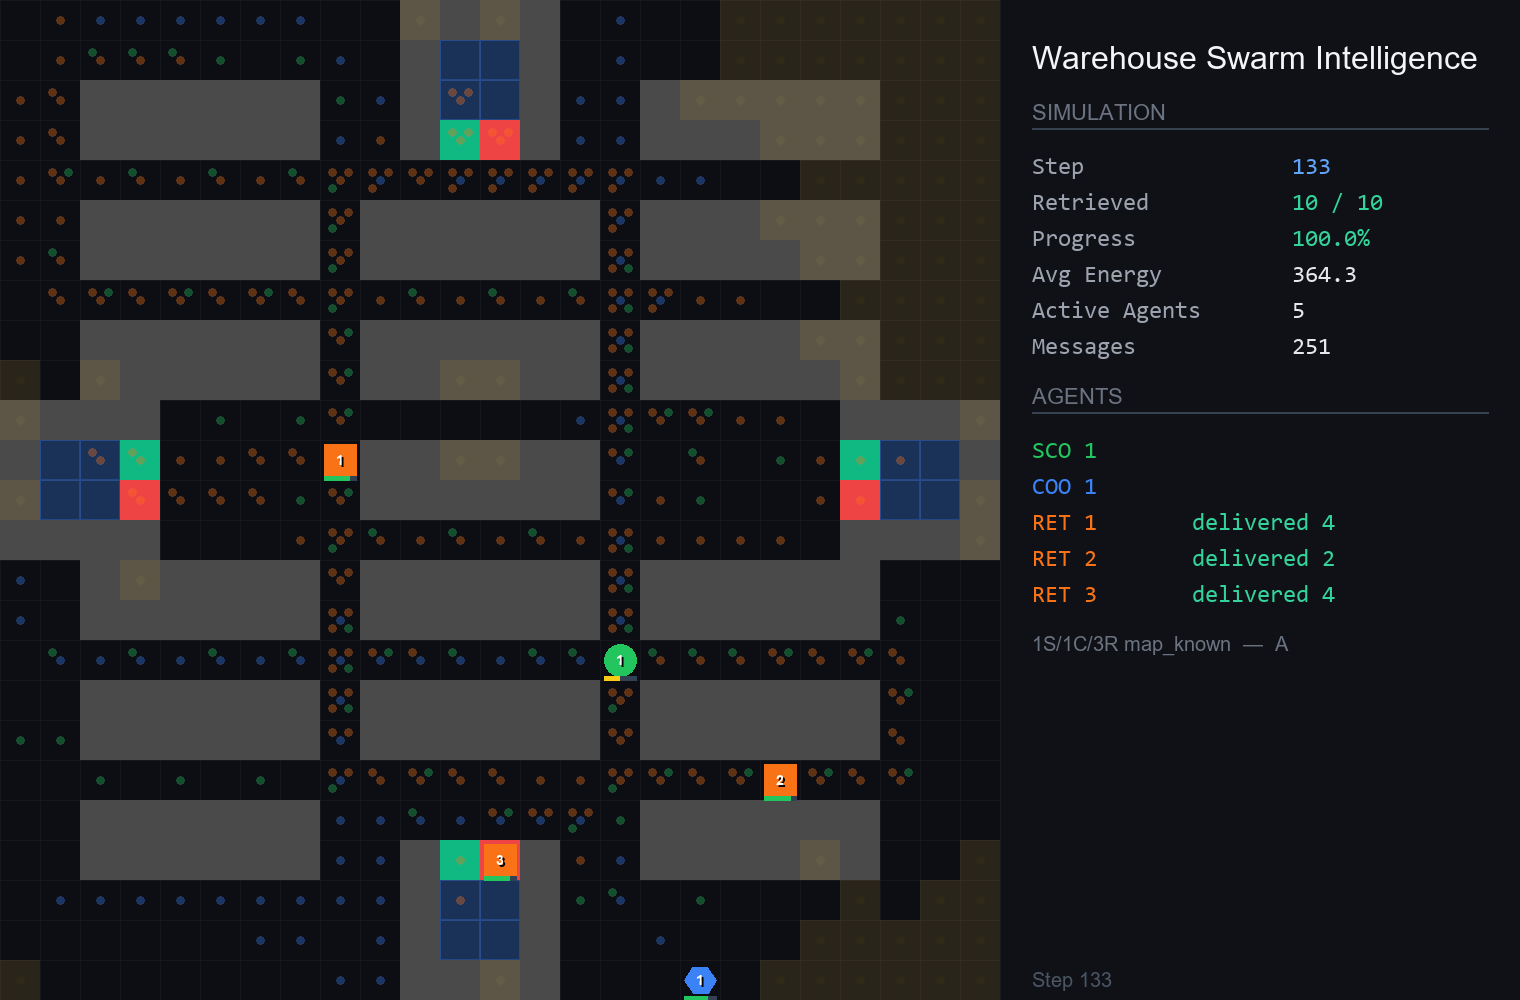
\includegraphics[width=0.48\textwidth]{../benchmarks/A/snapshot_1S-1C-3R_map_known.png}}%
  \hfill
  \subcaptionbox{1S-1C-3R --- \texttt{unknown}\label{fig:snap-a-13r-unk}}[0.48\textwidth]{%
    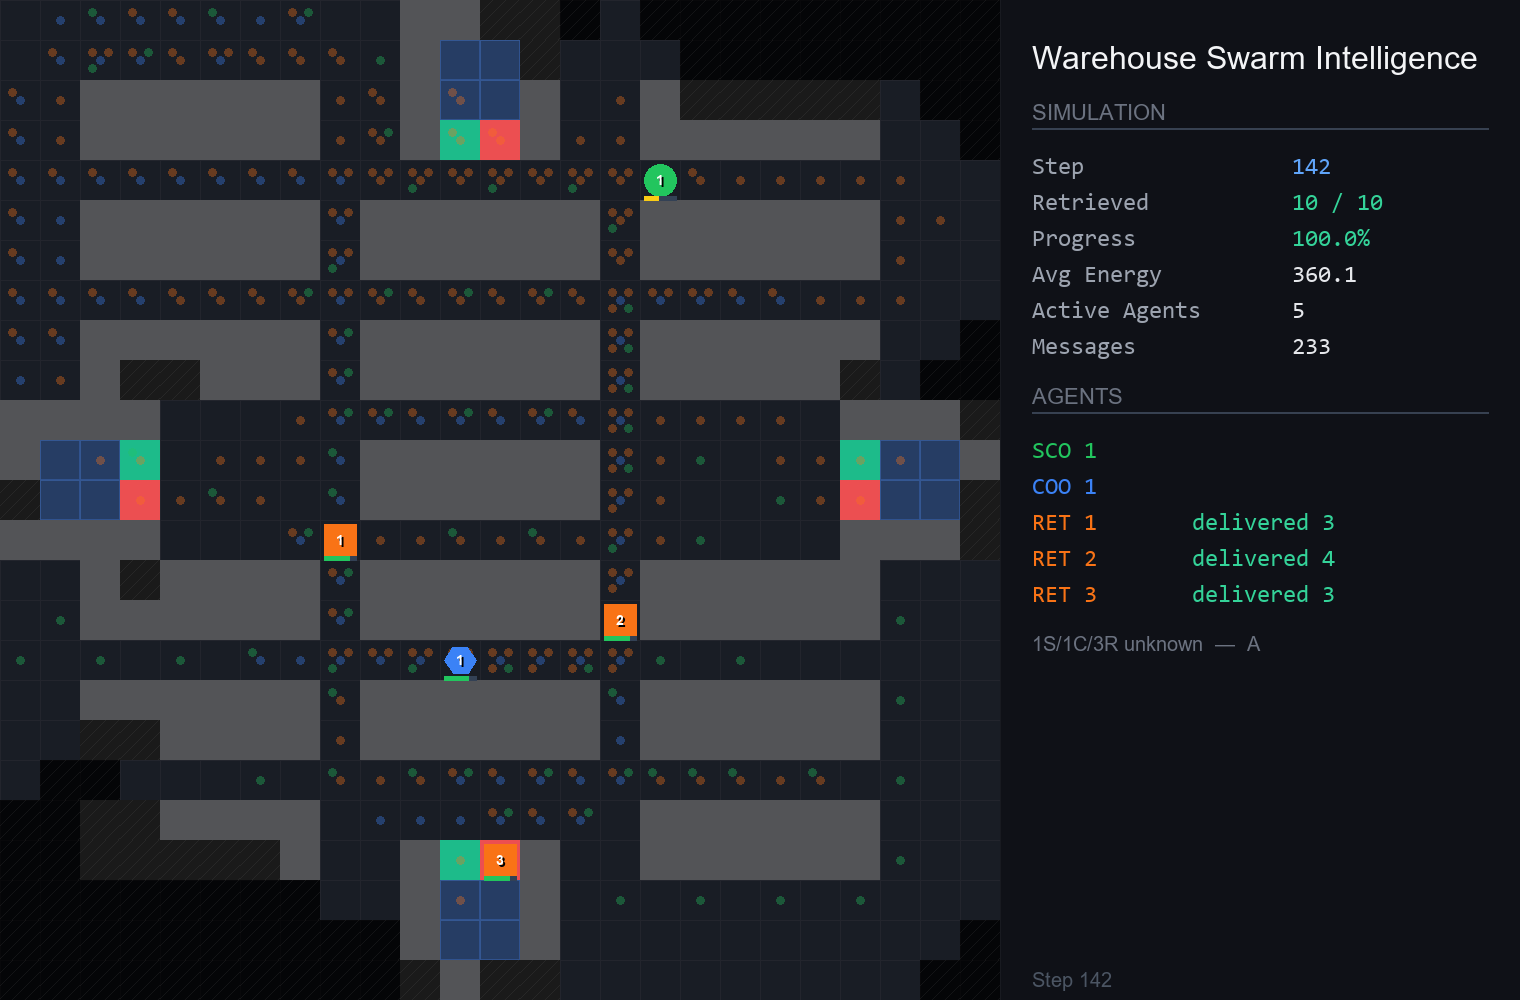
\includegraphics[width=0.48\textwidth]{../benchmarks/A/snapshot_1S-1C-3R_unknown.png}}%
  \\[1ex]
  \subcaptionbox{1S-1C-3R --- \texttt{map\_known}, $v_r\!=\!3,c_r\!=\!3$\label{fig:snap-a-13r-mk-v3c3}}[0.48\textwidth]{%
    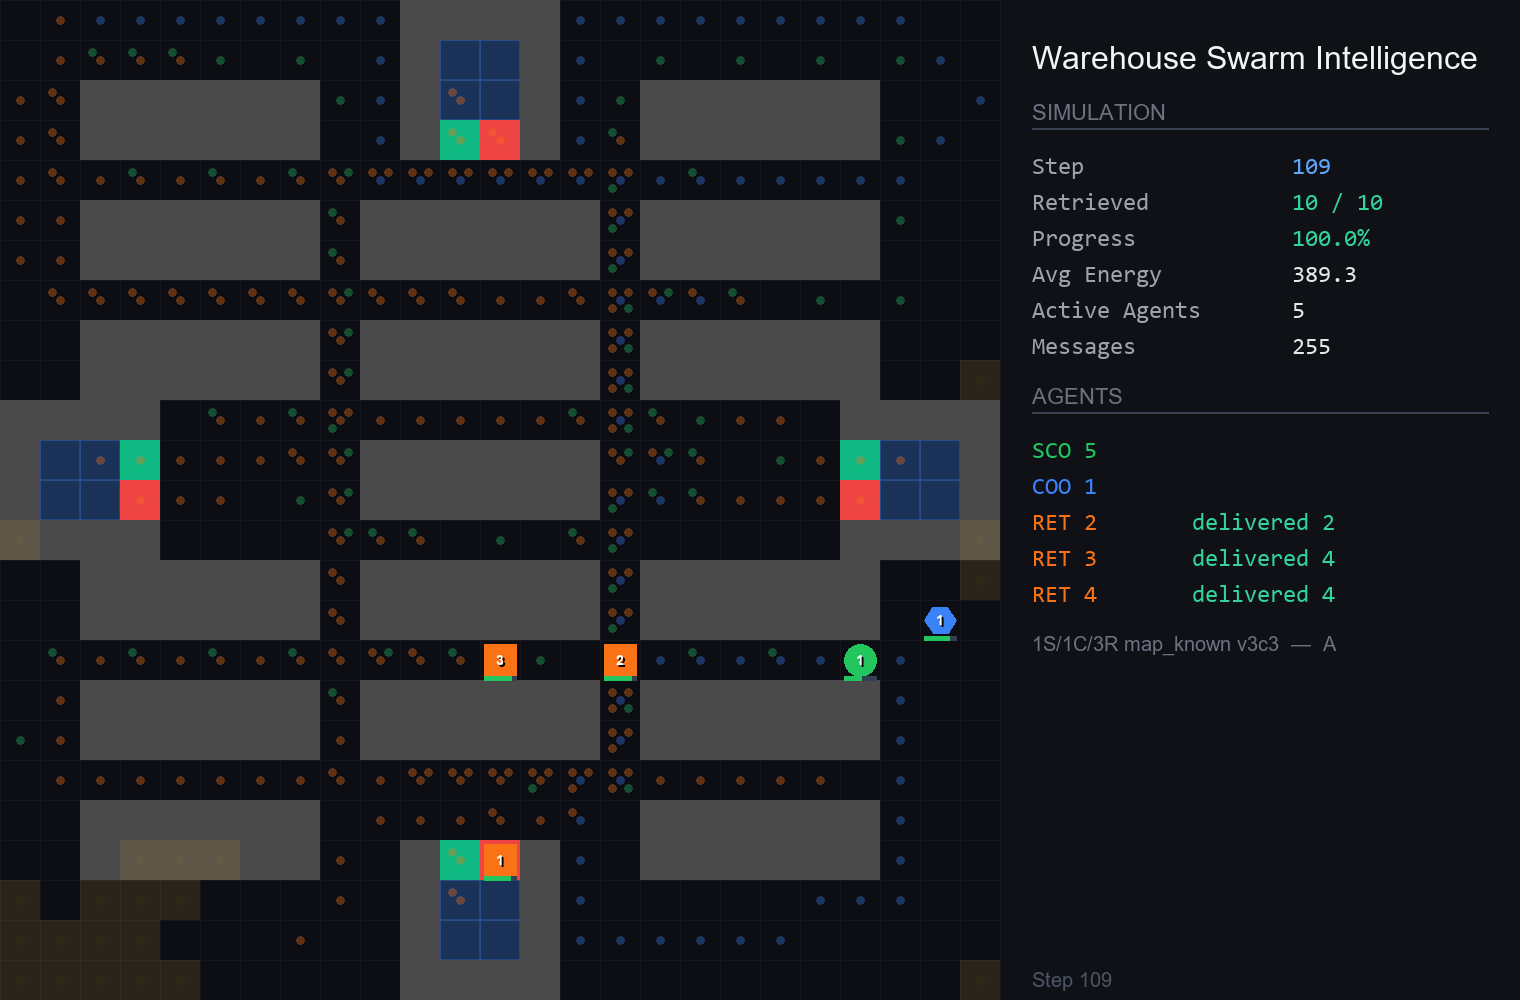
\includegraphics[width=0.48\textwidth]{../benchmarks/A/snapshot_1S-1C-3R_map_known_v3c3.png}}%
  \hfill
  \subcaptionbox{1S-1C-3R --- \texttt{unknown}, $v_r\!=\!3,c_r\!=\!3$\label{fig:snap-a-13r-unk-v3c3}}[0.48\textwidth]{%
    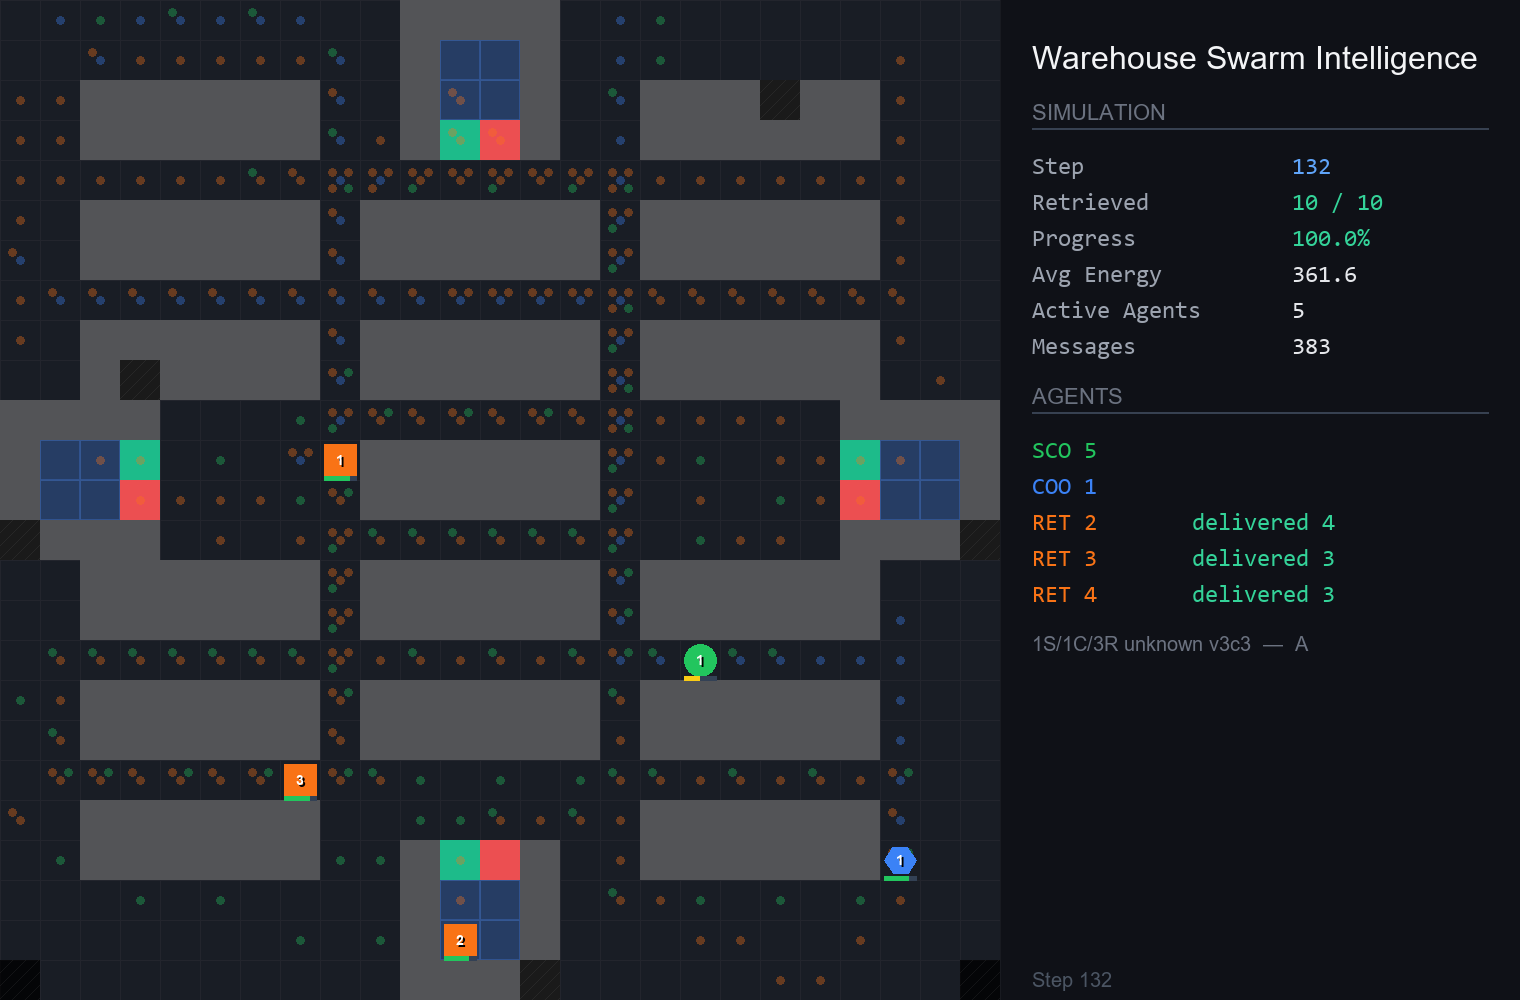
\includegraphics[width=0.48\textwidth]{../benchmarks/A/snapshot_1S-1C-3R_unknown_v3c3.png}}%
  \caption{Snapshot finali --- 1S-1C-3R, Preset~A}
  \label{fig:snap-a-13r}
\end{figure}

\begin{figure}[H]
  \centering
  \subcaptionbox{1S-1C-3R --- \texttt{map\_known}, no-seek\label{fig:snap-a-13r-mk-ns}}[0.48\textwidth]{%
    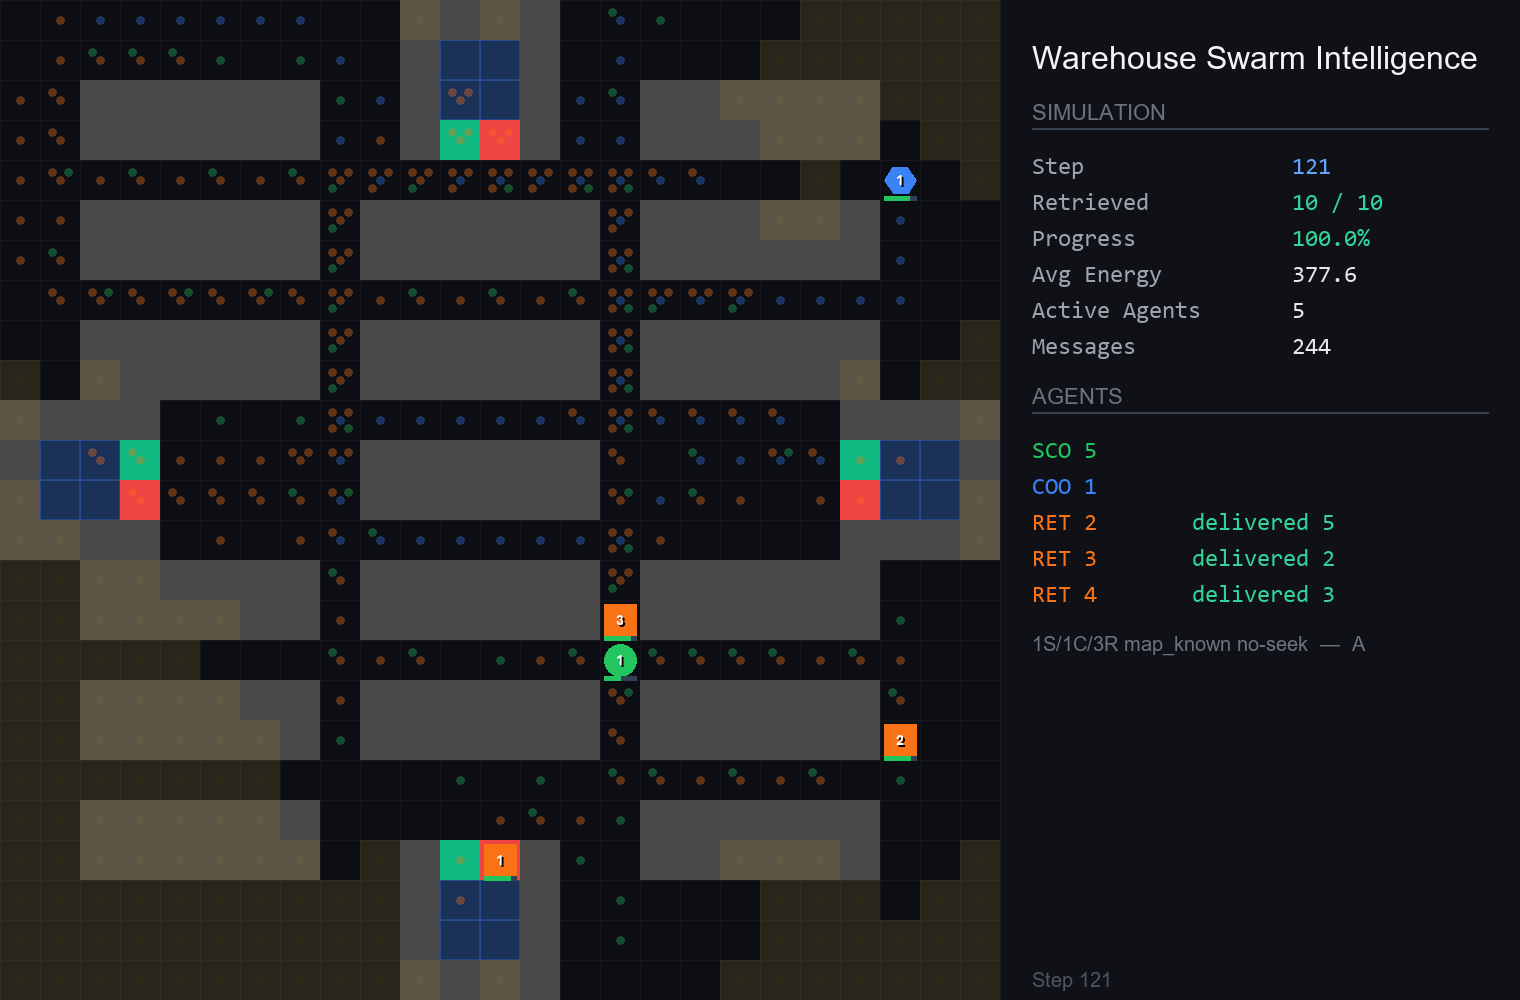
\includegraphics[width=0.48\textwidth]{../benchmarks/A/snapshot_1S-1C-3R_map_known_no-seek.png}}%
  \hfill
  \subcaptionbox{1S-1C-3R --- \texttt{unknown}, no-seek\label{fig:snap-a-13r-unk-ns}}[0.48\textwidth]{%
    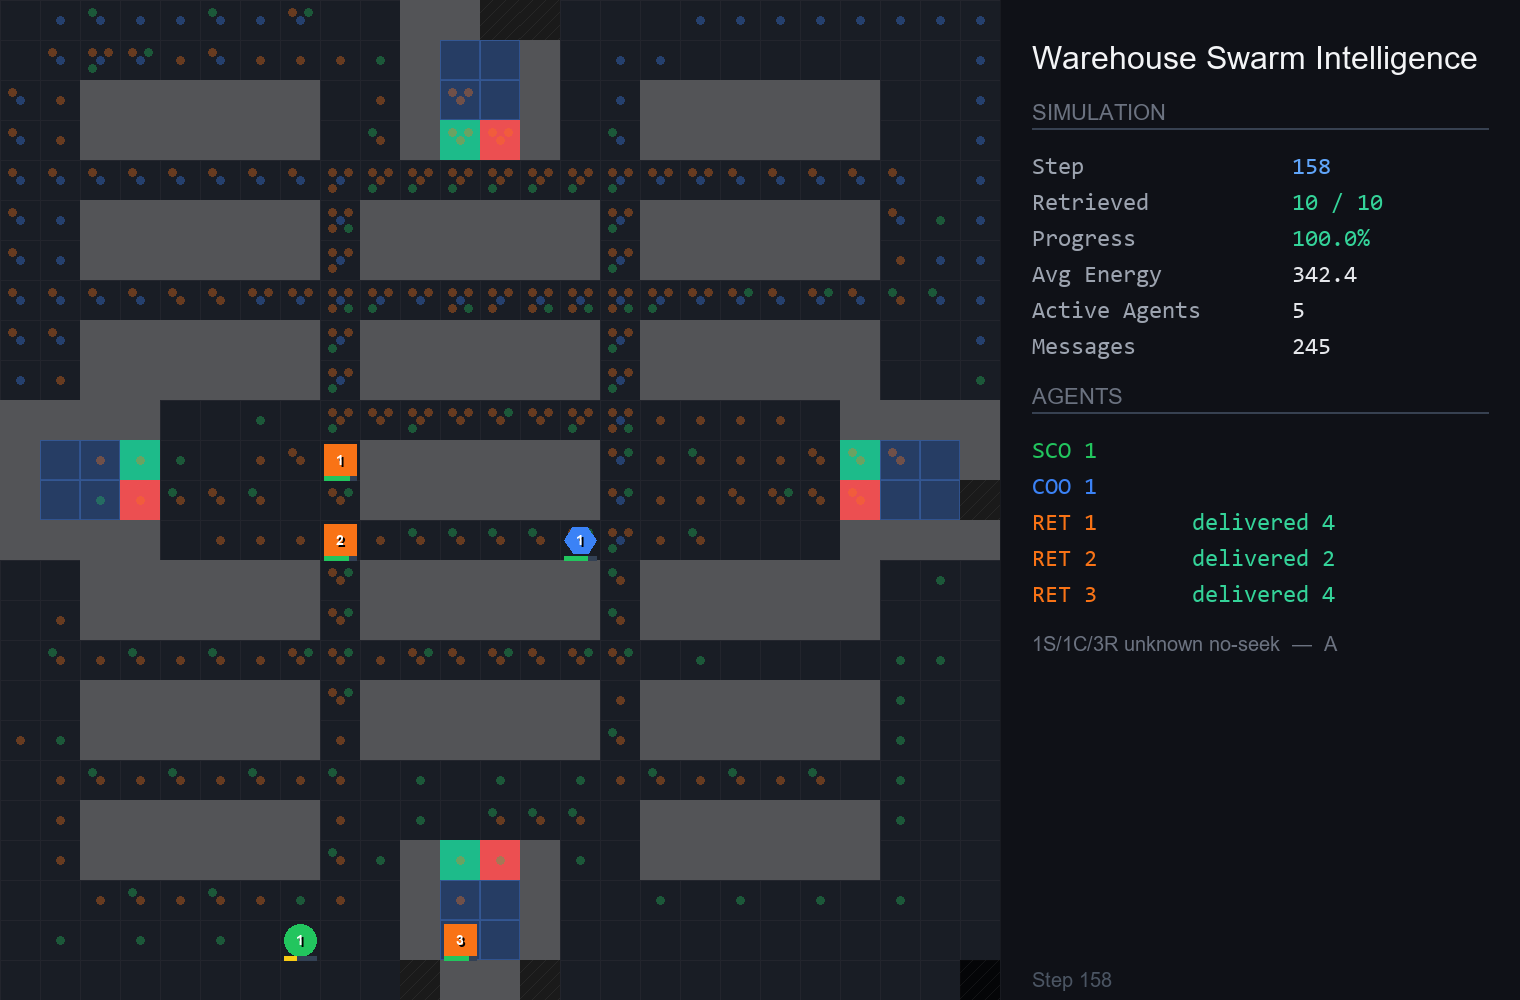
\includegraphics[width=0.48\textwidth]{../benchmarks/A/snapshot_1S-1C-3R_unknown_no-seek.png}}%
  \\[1ex]
  \subcaptionbox{1S-1C-3R --- \texttt{map\_known}, no-seek, $v_r\!=\!3,c_r\!=\!3$\label{fig:snap-a-13r-mk-ns-v3c3}}[0.48\textwidth]{%
    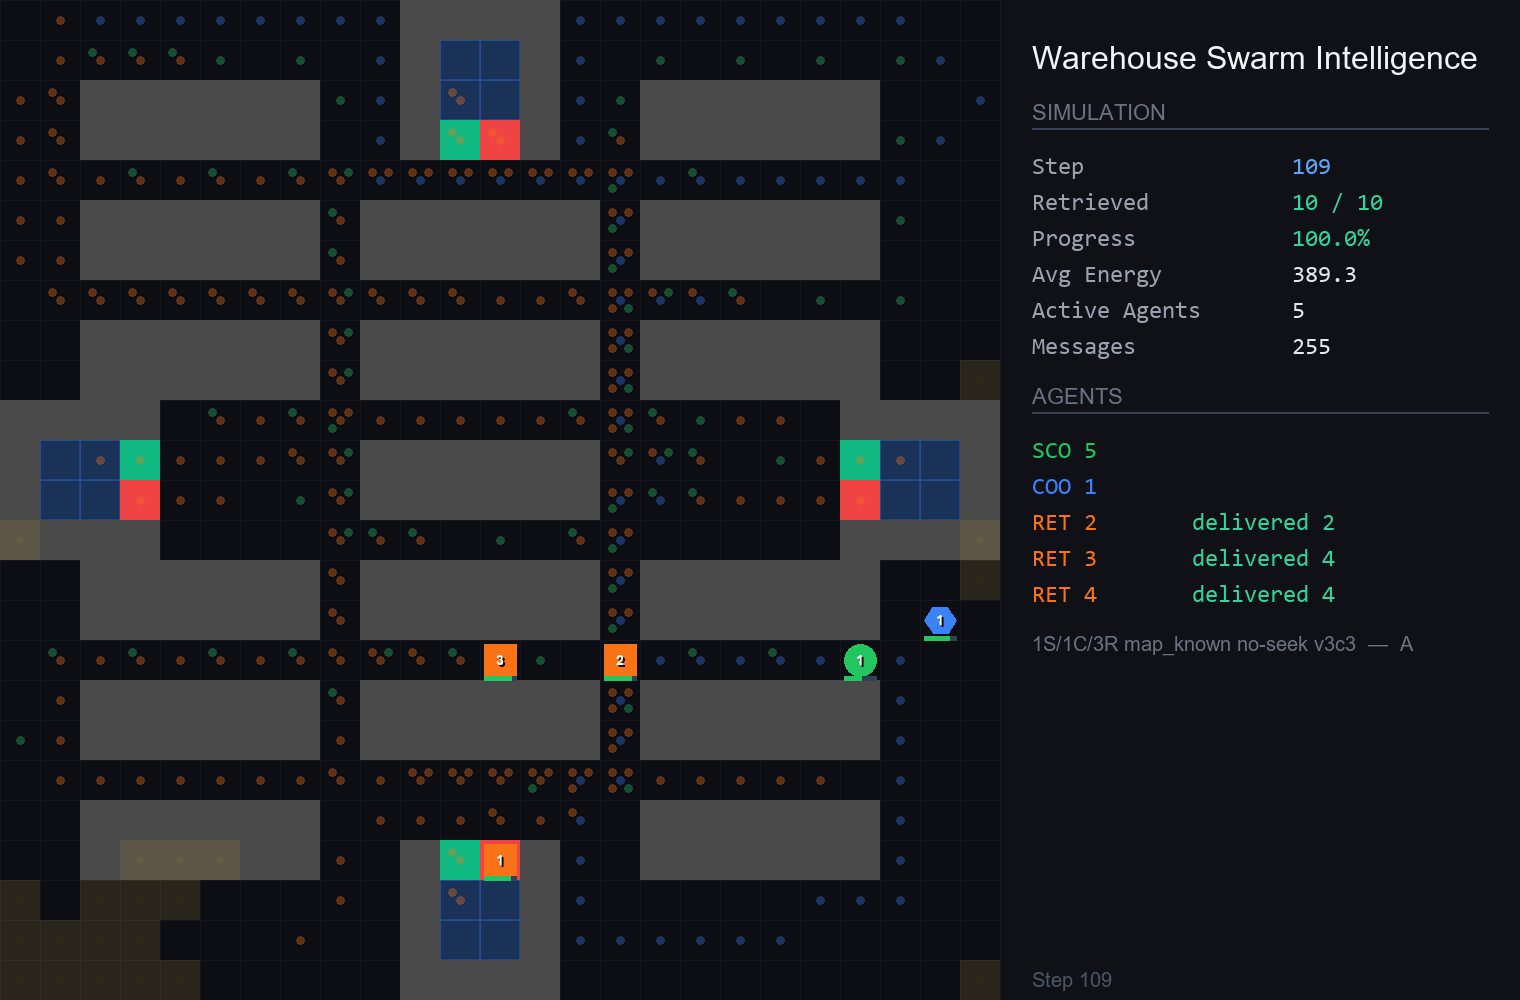
\includegraphics[width=0.48\textwidth]{../benchmarks/A/snapshot_1S-1C-3R_map_known_no-seek_v3c3.png}}%
  \hfill
  \subcaptionbox{1S-1C-3R --- \texttt{unknown}, no-seek, $v_r\!=\!3,c_r\!=\!3$\label{fig:snap-a-13r-unk-ns-v3c3}}[0.48\textwidth]{%
    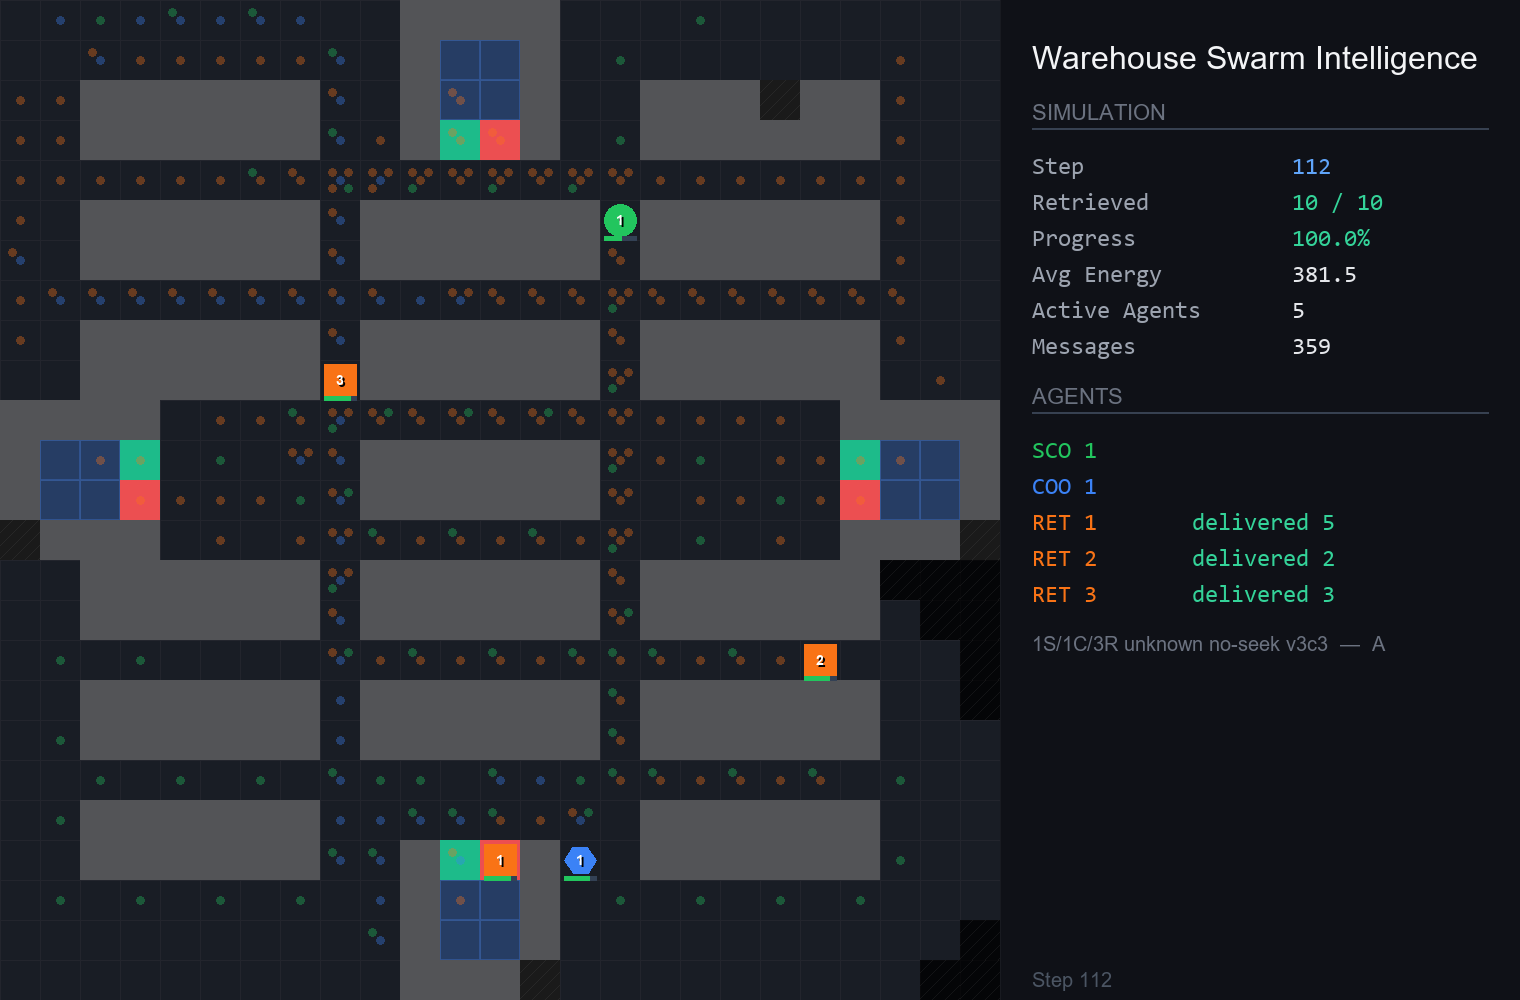
\includegraphics[width=0.48\textwidth]{../benchmarks/A/snapshot_1S-1C-3R_unknown_no-seek_v3c3.png}}%
  \caption{Snapshot finali --- 1S-1C-3R no-seek, Preset~A}
  \label{fig:snap-a-13r-ns}
\end{figure}

%% ── Preset B ──────────────────────────────────────────────
\section{Preset B}

\begin{figure}[H]
  \centering
  
\includegraphics[width=\textwidth]{../benchmarks/B/retrieval.png}
  \caption{Andamento del recupero oggetti --- Preset~B}
  \label{fig:bench-b-retrieval}
\end{figure}

\begin{figure}[H]
  \centering
  
\includegraphics[width=\textwidth]{../benchmarks/B/energy.png}
  \caption{Consumo energetico --- Preset~B}
  \label{fig:bench-b-energy}
\end{figure}

\begin{figure}[H]
  \centering
  
\includegraphics[width=\textwidth]{../benchmarks/B/efficiency.png}
  \caption{Efficienza energetica --- Preset~B}
  \label{fig:bench-b-efficiency}
\end{figure}

\begin{figure}[H]
  \centering
  
\includegraphics[width=\textwidth]{../benchmarks/B/messages.png}
  \caption{Messaggi scambiati --- Preset~B}
  \label{fig:bench-b-messages}
\end{figure}

\begin{figure}[H]
  \centering
  
\includegraphics[width=\textwidth]{../benchmarks/B/steps_comparison.png}
  \caption{Confronto step totali --- Preset~B}
  \label{fig:bench-b-steps}
\end{figure}

\begin{figure}[H]
  \centering
  
\includegraphics[width=0.92\textwidth]{../benchmarks/B/summary_table.png}
  \caption{Tabella riepilogativa --- Preset~B}
  \label{fig:bench-b-table}
\end{figure}

\subsection{Snapshot Finali --- Preset~B}

\begin{figure}[H]
  \centering
  \subcaptionbox{0S-0C-5R --- \texttt{map\_known}\label{fig:snap-b-05r-mk}}[0.48\textwidth]{%
    
\includegraphics[width=0.48\textwidth]{../benchmarks/B/snapshot_0S-0C-5R_map_known.png}}%
  \hfill
  \subcaptionbox{0S-0C-5R --- \texttt{unknown}\label{fig:snap-b-05r-unk}}[0.48\textwidth]{%
    
\includegraphics[width=0.48\textwidth]{../benchmarks/B/snapshot_0S-0C-5R_unknown.png}}%
  \\[1ex]
  \subcaptionbox{0S-0C-5R --- \texttt{map\_known}, $v_r\!=\!3,c_r\!=\!3$\label{fig:snap-b-05r-mk-v3c3}}[0.48\textwidth]{%
    
\includegraphics[width=0.48\textwidth]{../benchmarks/B/snapshot_0S-0C-5R_map_known_v3c3.png}}%
  \hfill
  \subcaptionbox{0S-0C-5R --- \texttt{unknown}, $v_r\!=\!3,c_r\!=\!3$\label{fig:snap-b-05r-unk-v3c3}}[0.48\textwidth]{%
    
\includegraphics[width=0.48\textwidth]{../benchmarks/B/snapshot_0S-0C-5R_unknown_v3c3.png}}%
  \caption{Snapshot finali --- 0S-0C-5R, Preset~B}
  \label{fig:snap-b-05r}
\end{figure}

\begin{figure}[H]
  \centering
  \subcaptionbox{1S-1C-3R --- \texttt{map\_known}\label{fig:snap-b-13r-mk}}[0.48\textwidth]{%
    
\includegraphics[width=0.48\textwidth]{../benchmarks/B/snapshot_1S-1C-3R_map_known.png}}%
  \hfill
  \subcaptionbox{1S-1C-3R --- \texttt{unknown}\label{fig:snap-b-13r-unk}}[0.48\textwidth]{%
    
\includegraphics[width=0.48\textwidth]{../benchmarks/B/snapshot_1S-1C-3R_unknown.png}}%
  \\[1ex]
  \subcaptionbox{1S-1C-3R --- \texttt{map\_known}, $v_r\!=\!3,c_r\!=\!3$\label{fig:snap-b-13r-mk-v3c3}}[0.48\textwidth]{%
    
\includegraphics[width=0.48\textwidth]{../benchmarks/B/snapshot_1S-1C-3R_map_known_v3c3.png}}%
  \hfill
  \subcaptionbox{1S-1C-3R --- \texttt{unknown}, $v_r\!=\!3,c_r\!=\!3$\label{fig:snap-b-13r-unk-v3c3}}[0.48\textwidth]{%
    
\includegraphics[width=0.48\textwidth]{../benchmarks/B/snapshot_1S-1C-3R_unknown_v3c3.png}}%
  \caption{Snapshot finali --- 1S-1C-3R, Preset~B}
  \label{fig:snap-b-13r}
\end{figure}

\begin{figure}[H]
  \centering
  \subcaptionbox{1S-1C-3R --- \texttt{map\_known}, no-seek\label{fig:snap-b-13r-mk-ns}}[0.48\textwidth]{%
    
\includegraphics[width=0.48\textwidth]{../benchmarks/B/snapshot_1S-1C-3R_map_known_no-seek.png}}%
  \hfill
  \subcaptionbox{1S-1C-3R --- \texttt{unknown}, no-seek\label{fig:snap-b-13r-unk-ns}}[0.48\textwidth]{%
    
\includegraphics[width=0.48\textwidth]{../benchmarks/B/snapshot_1S-1C-3R_unknown_no-seek.png}}%
  \\[1ex]
  \subcaptionbox{1S-1C-3R --- \texttt{map\_known}, no-seek, $v_r\!=\!3,c_r\!=\!3$\label{fig:snap-b-13r-mk-ns-v3c3}}[0.48\textwidth]{%
    
\includegraphics[width=0.48\textwidth]{../benchmarks/B/snapshot_1S-1C-3R_map_known_no-seek_v3c3.png}}%
  \hfill
  \subcaptionbox{1S-1C-3R --- \texttt{unknown}, no-seek, $v_r\!=\!3,c_r\!=\!3$\label{fig:snap-b-13r-unk-ns-v3c3}}[0.48\textwidth]{%
    
\includegraphics[width=0.48\textwidth]{../benchmarks/B/snapshot_1S-1C-3R_unknown_no-seek_v3c3.png}}%
  \caption{Snapshot finali --- 1S-1C-3R no-seek, Preset~B}
  \label{fig:snap-b-13r-ns}
\end{figure}
